\documentclass[12pt]{article}
\usepackage{graphicx}

\title{Notes on transient mortality shocks in low-mortality populations}
\author{Joshua R. Goldstein \and Ronald D. Lee}

\begin{document}

\maketitle
\begin{abstract}
  Here we present preliminary results for the modeling of transient mortality shocks
  based on Lee-Carter estimates of the evolution of mortality over
  time. The model we fit includes random terms for the evolution of
  the underlying trend, which is modeled as a random walk with
  deterministic drift, and for transient shocks, which we interpret
  as single-year events due to weather or annual infectious diseases
  like the flu. These preliminary models only work well for some
  countries. Nonetheless it is still possible to see that the
  transient shocks of neighbors are correlated, suggesting that they
  are picking up real variation in mortality, rather than measurement
  error.
\end{abstract}

\section{Overview}


The canonical time-series model used for the Lee-Carter model is the
random walk with drift. The logic behind this is that there is a
steady march of progress toward lower mortality which varies in its
pace. The recent three-year run of declining mortality in the United
States -- and the current pandemic -- suggest that there are
short-term factors other than technological progress and changes in
population health that may be important for mortality in any given
year.

Modeling these short-term transient shocks is interesting in its own
right, because of what it reveals about the nature of population
mortality levels and changes.  It may also be useful for understanding
the long-run implications of mortality reversals like that from the
U.S. opioid crisis or the worldwide coronavirus pandemic.


Here we present preliminary results for the modeling of transient
mortality shocks based on Lee-Carter estimates of the evolution of
mortality over time. The model we fit includes random terms for the
evolution of the underlying trend, which is modeled as a random walk
with deterministic drift, and for transient shocks, which we interpret
as single-year events due to weather or annual infectious diseases
like the flu.

These preliminary models only work well for some
countries. Nonetheless it is still possible to see that the transient
shocks of neighbors are correlated, suggesting that they are picking
up real variation in mortality, rather than measurement error.


\section{Modeling}

We first estimate the Lee-Carter model, adjusting $k_t$ to match
$e_0$. This model reduces the logarithm of the full set of age-period
mortality rates to an average age-schedule $a_x$ and a time index $k_t$ that
drives age-specific changes $b_x$. The model has the form
$$
\log M_{x,t} = a_x + b_x k_t.
$$
Standard methods are available for estimating the parameters.

The usual time series model for forecasting is the random walk with
drift
$$
k_t = k_{t-1} + d + \epsilon_t.
$$

Here we add another layer to the estimation of the time series,
decomposing the observed $k_t$ into a latent $k_t$ that evolves as a
random walk with drift and an annual transitory component $n_t$. In
state-space modeling $n_t$ is sometimes called ``observation
error'' or ``noise''. We are conceiving of it not so much as error but as a
transitory perturbation -- for example due to weather or the severity
of the annual flu or to another kind of contagious disease such as
COVID-19.

The model has the form

\begin{equation}
  k_t^{observed} = k_t^{latent} + n_t
\end{equation}

\begin{equation}
  k_t^{latent} = k_{t-1}^{latent} + d + \epsilon_t
\end{equation}

The model has two features.
\begin{itemize}
  \item The observed value is the latent value plus ``noise'' $n_t$,
    which is assumed to be normally distributed with constant variance
    and independent over $t$.

  \item The latent value evolves as a random walk with drift, with a
    fixed (deterministic) value of $d$.

\end{itemize}

Note it is also possible to add an additional random layer to this
model by making $d$ itself a stochastic evolving term. The
standard form of this ``random trend'' model is to let $d$ evolve as a
random walk, $d_t = d_{t-1} + \eta_{t-1}$. We don't consider this
model for now.

\section{Results}

In Figure \ref{kt_panel_fig} we show the observed and latent $k_t$ for
9 countries in the Human Mortality Database. In some countries, such
as the United States, Russia, and West Germany, the latent level of
mortality is indistinguishable from the observed level. In the others, 
latent value is clearly a smoother version of the observed $k_t$. The
smoothing is particularly evident in France, Spain, and Sweden. Italy
and Japan are intermediate cases.

\begin{figure}

  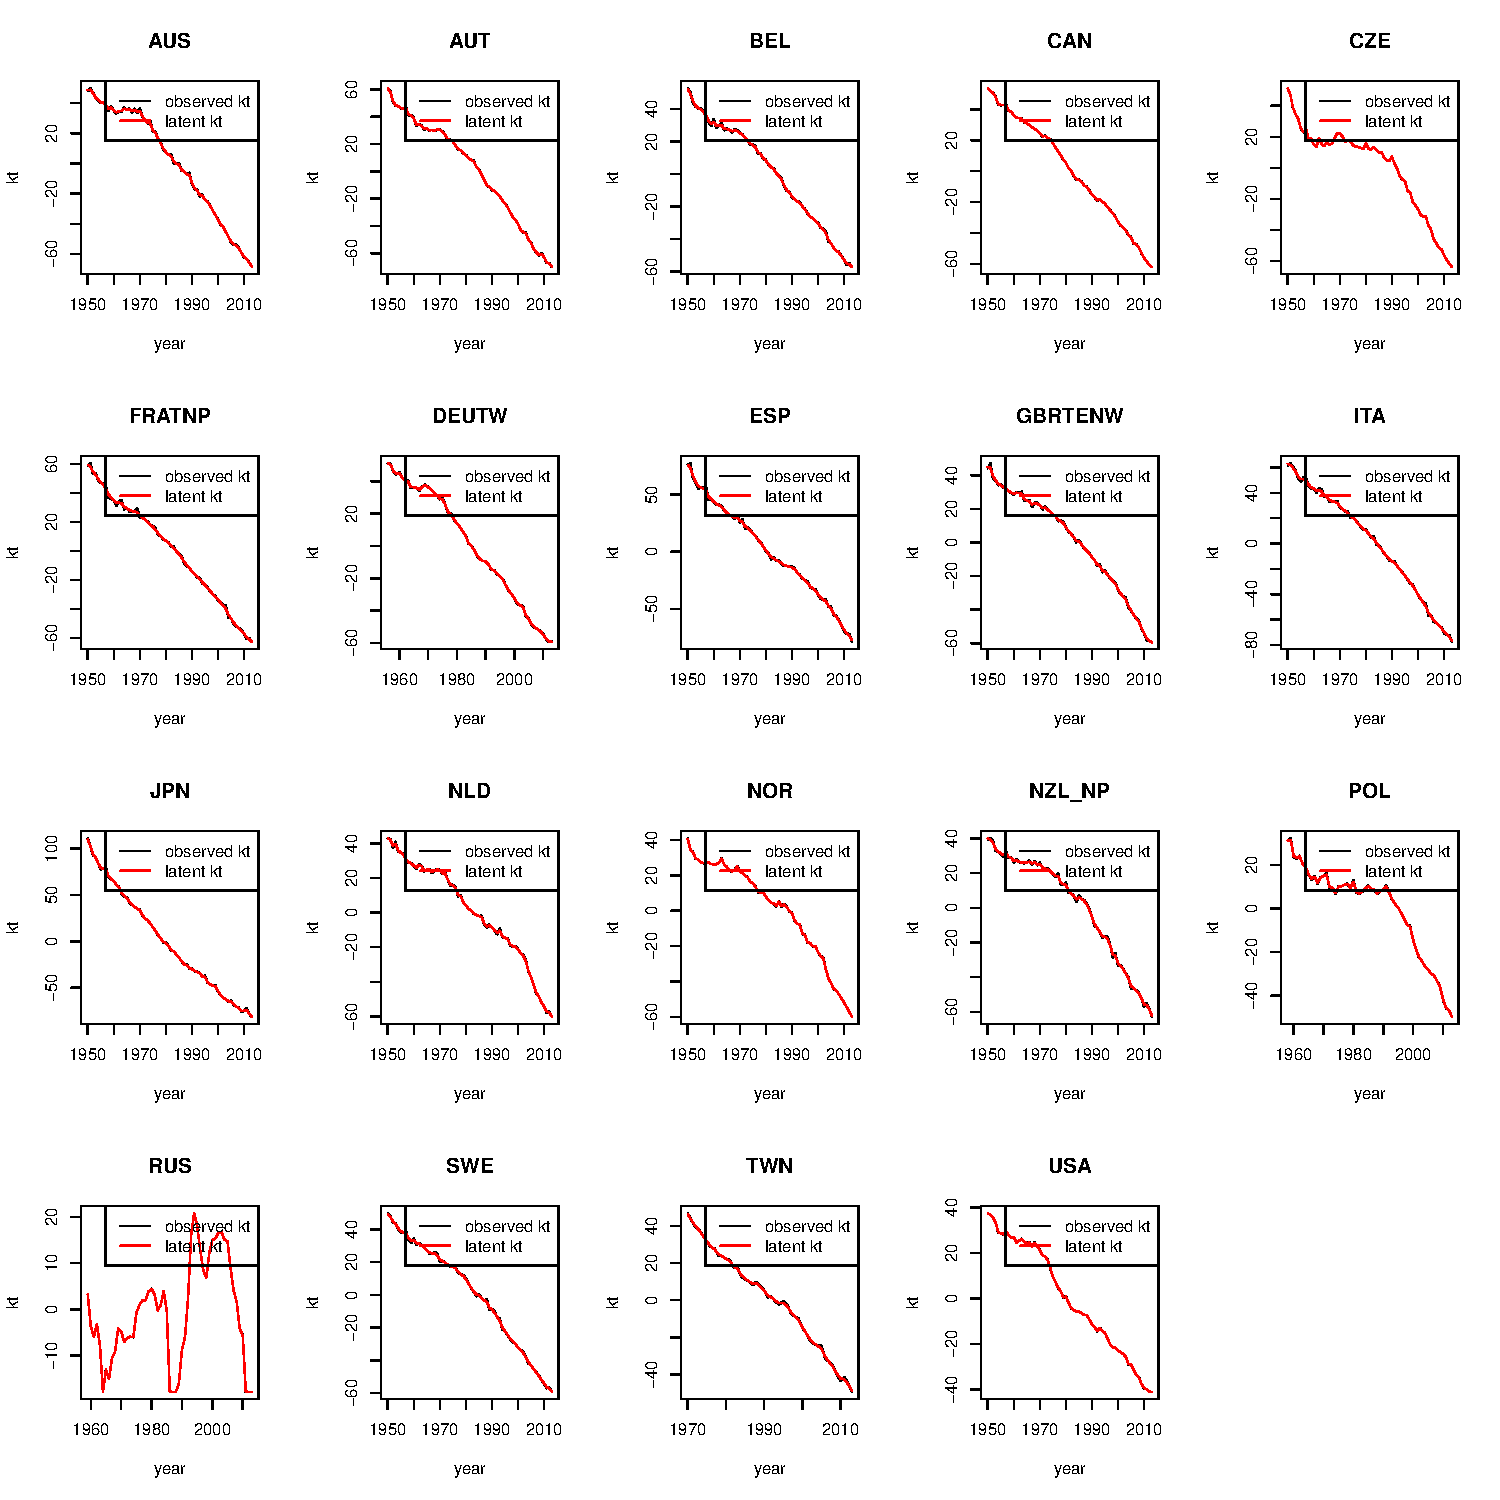
\includegraphics[width=1.05\textwidth]{./kt_panel_fig.pdf}
  \caption{Estimates of observed and latent values of $k_t$ in
    Lee-Carter model using MARSS package based on HMD data. Zoom in to
    see detail. Take home: In some countries (e.g., Sweden, France,
    Spain, and the UK), the estimation gives a much smoother latent
    value. In the USA this model doesn't produce much of interest.}
    \label{kt_panel_fig}
\end{figure}


The contrast between countries can be seen more clearly in Figure
\ref{kt_recent_panel_fig}, which shows the same estimates as in Figure
\ref{kt_panel_fig} but only since 1990.

\begin{figure}

  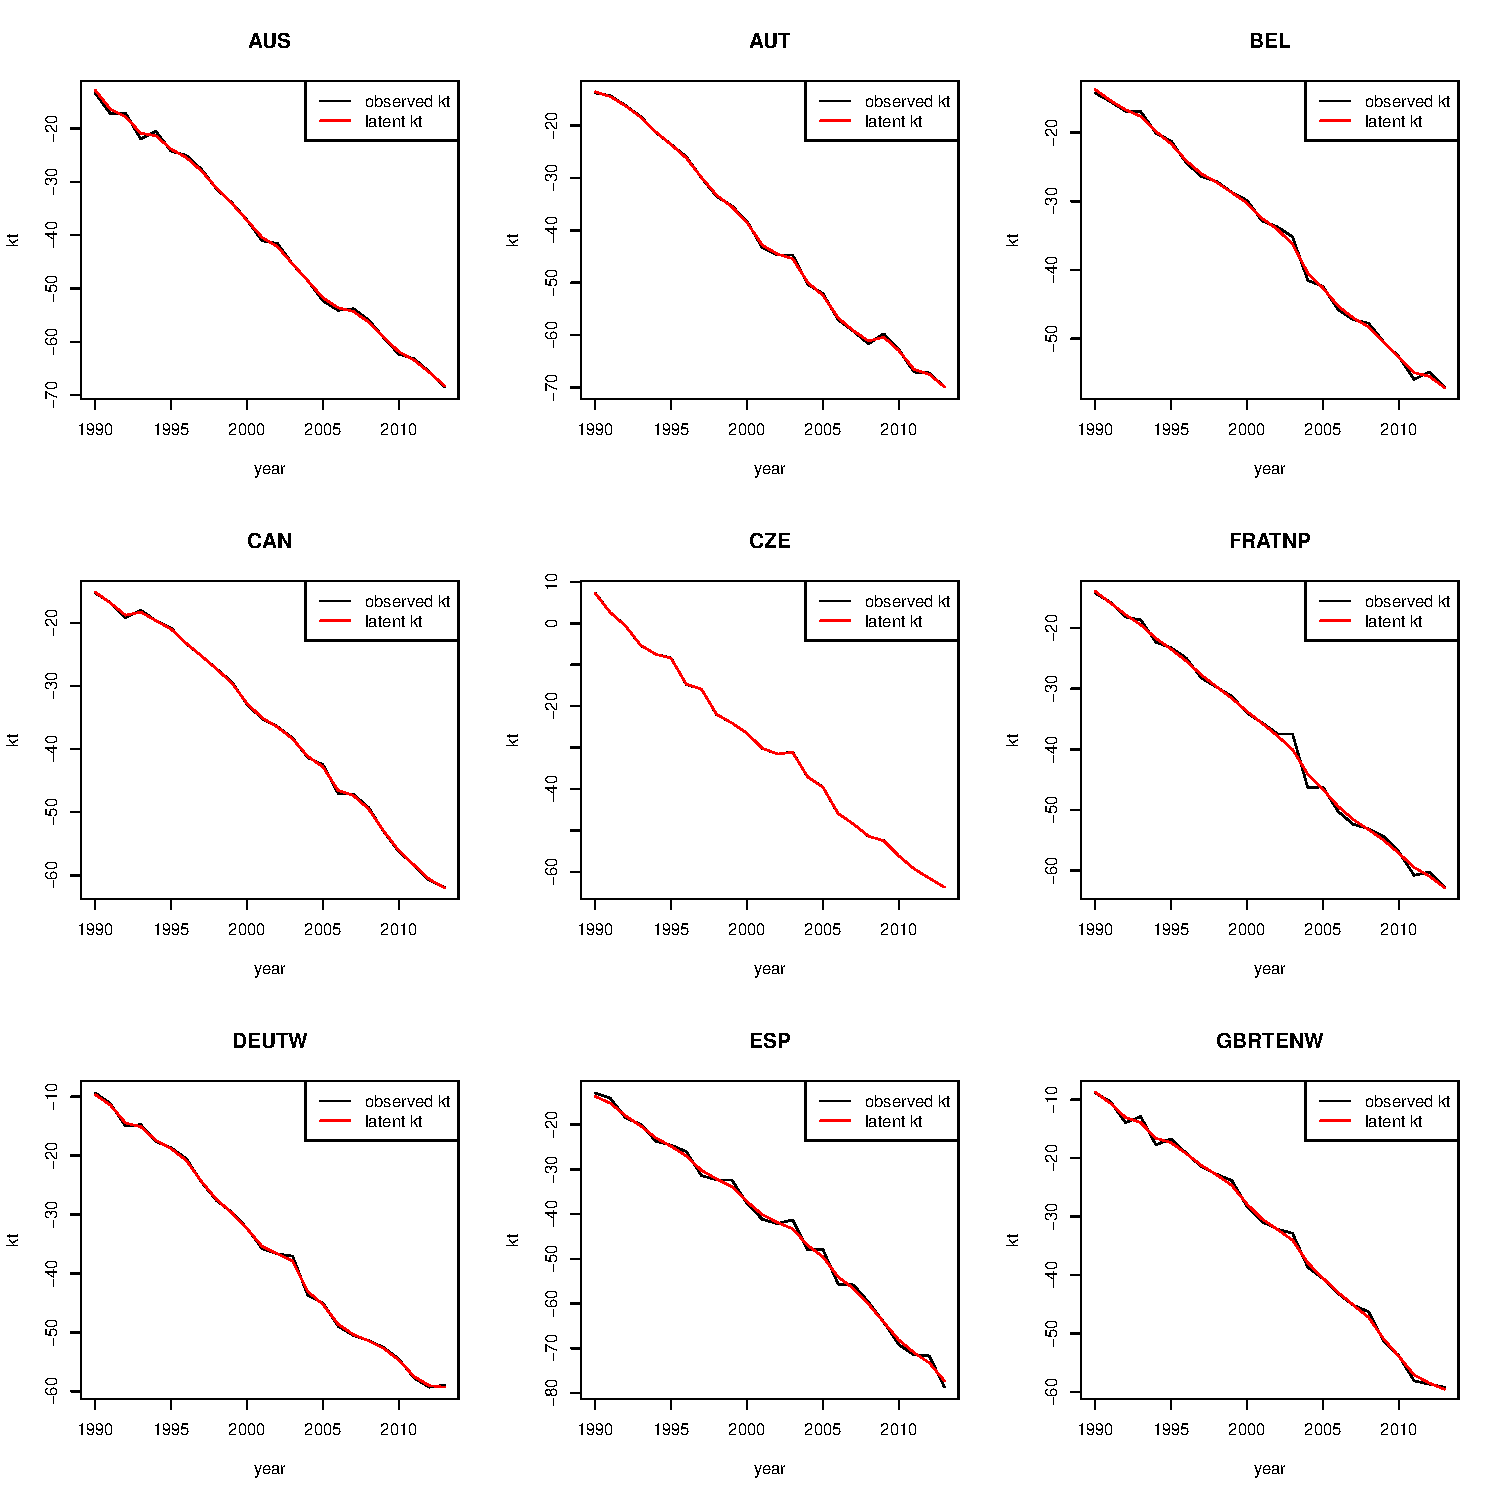
\includegraphics[width=1.05\textwidth]{./kt_recent_panel_fig.pdf}
  \caption{Zoomed in version of Figure \ref{kt_panel_fig}, showing
    results since 1990.}
    \label{kt_recent_panel_fig}
\end{figure}


Figure \ref{kt_resid_panel_fig} shows the estimated values of $n_t$
(the difference between observed and latent $k_t$). These can be
interpreted as the transitory shocks (and/or measurement error). The
plots are done on the same scale. The large values are associated with
countries in which there is a lot of smoothing.

\begin{figure}
  \label{kt_resid_panel_fig}
  \includegraphics[width=1.05\textwidth]{./kt_resid_panel_fig.pdf}
  \caption{Estimated shocks $n_t = k_t^{latent} - k_t^{observed}$,
    shown on a common scale.}
\end{figure}


Finally, \ref{nt_pairs_fig} shows how the ``noise'' $n_t$ is
correlated for neighboring countries. (Note: The scale differs by
plot). We can see very high correlations between Italy and France
(0.76) and very low correlations between the UK and Japan (0.13).

\begin{figure}
  \label{nt_pairs_fig}
  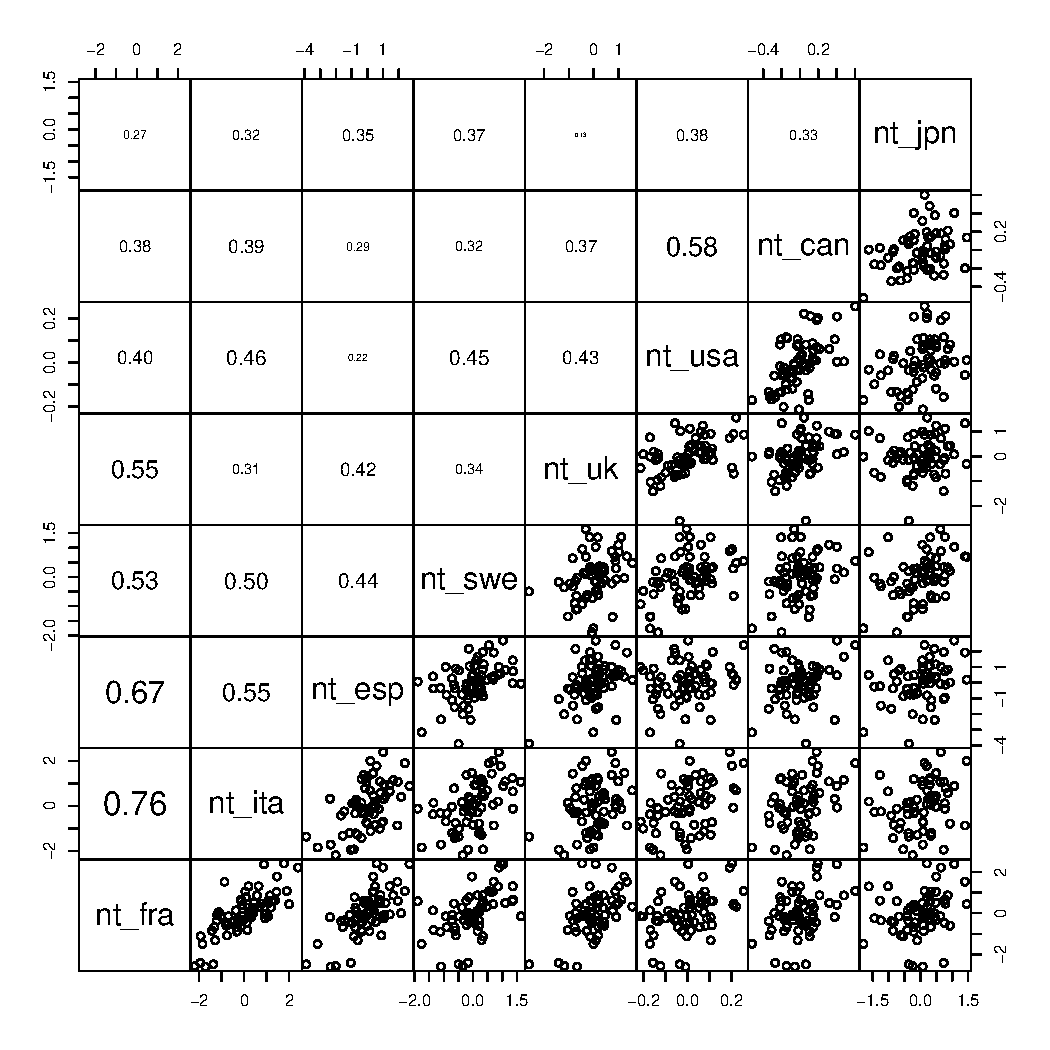
\includegraphics[width=1.05\textwidth]{./nt_pairs.pdf}
  \caption{Correlations across countries in the time series of
    $n_t(country)$. Note strong correlations between Spain, France,
    and Italy -- and also the USA and Canada.}
\end{figure}


Interestingly, we see that Italy, Spain, and France are all closely
related. So are the United States and Canada. Sweden in the United
States are also similar. 


\section{Discussion}

Our estimation of transitory mortality is not complete. But a few
preliminary conclusions can be reached

\begin{enumerate}

  \item In some countries, the observed $k_t$ is noticeably more
    volatile than the latent $k_t$. In these cases, it might be
    preferable to begin forecasts at the most recent value of the
    latent $k_t$. One might also want to use the estimated variances
    of $\epsilon_t$ and $n_t$ to estimate forecast uncertainty.

  \item The ``noise'' we are estimating is correlated for neighboring
    countries. This makes it appear that there are weather and
    infectious diseases ``shocks'' that are shared across
    countries. It also makes it unlikely that measurement issues are
    behind the shocks.

  \item This simple model does not seem to apply to United States,
    where the latent and observed $k_t$ are indistinguishable. This is
    consistent with Lawrence Carter's paper, showing that structural
    time series forecasts for the US are nearly the same as ARIMA


\end{enumerate}

\section{Future directions}

Future steps to be taken could include

\begin{enumerate}

  \item Check on convergence, measures of model fit and so forth for
    all of these countries. (The estimates shown should be considered
    preliminary.)

  \item Check to see if making the drift term stochastic makes a
    difference in countries like Sweden or France. This is not
    possible using the same software that I'm using. But it is easy to
    estimate with other software. I suspect that the drift term will
    have almost no stochastic variation, because the time series
    already look very linear.

  \item Figure out how to get more meaningful estimates of  $n_t$ for the
    United States and other countries where estimation of the latent
    $k_t$ doesn't produce much of interest. One way to do this might
    be to change the assumptions about the statistical distribution of
    $n_t$. For example, it could have heavier tails (which is one way
    to make it more sporadic). Doing this requires other software, but
    I think I use a Bayesian approach for estimating all of the models
    using a consistent method.

  \item It might be interesting to include more countries and show how
    shocks are correlated. (In Asia, we can add Taiwan, Korea and
    HK). In Europe there are many more countries. And we can add NZ
    and Australia.

  \item It might be interesting to do a kind of ``coherent'' forecast
    in which correlation of the $n(t)$ by country are taken into
    account. Perhaps there is also correlation of the $\epsilon(t)$?

  \item It would be interesting to see how much difference it makes to
    forecast with this latent model rather than the observed $k_t$. We
    could take a country like France or Sweden where there appears to
    be a difference and show how the forecast would have evolved over
    time, particularly for launch years which show a large gap between
    the observed and the latent $k(t)$ values.

\end{enumerate}

\end{document}


    